\section{The Network Layer}
\begin{itemize}

\item
In this chapter, we'll make an important distinction between the \textbf{forwarding} and \textbf{routing} functions of the network layer. Forwarding involves the transfer of a packet from an incoming link to an outgoing link within a \textit{single} router. Routing involves \textit{all} of a network's routers, whose collective interactions via routing protocols determines the paths that packets take on their trips from source to destination node.

\item
\textit{Forwarding} refers to the router-local action of transferring a packet from an input interface to the appropriate output link interface. \textit{Routing} refers to the network-wide process that determines the end-to-end paths that packets take from source to destination.

\item
We'll reserve the term \textit{packet switch} to mean a general packet-switching device that transfers a packet from input link interface to output link interface, according to the value in a field in the header of the packet. Some packet switches, called \textbf{link-layer switches}, base their forwarding decision on values in the fields of the link-layer frames; switches are thus referred to as link-layer (layer 2) devices. Other packet switches, called \textbf{routers}, base their forwarding decision on the value in the network-layer field. Routers are thus network-layer (layer 3) devices, but must also implement layer 2 protocols as well, since layer 3 devices require the services of layer 2 to implement their (layer 3) functionality.

\item
In an analogous manner, some network-layer architectures---for example, ATM, frame delay, and MPLS---require the routers along the chosen path from source to destination to handshake with each other in order to set up state before network-layer data packets within a given source-to-destination connection can begin to flow. In the network layer, this process is referred to as \textit{connection setup}.

\item
The Internet's network layer provides a single service, known as \textbf{best-effort service}.

\item
Two of the more important ATM service models are constant bit rate and available bit rate service:
\begin{itemize}
\item\textit{\textbf{Constant bit rate (CBR) ATM network service.}}
\item\textit{\textbf{Available bit rate (ABR) ATM network service.}}
\end{itemize}

\item
In a similar manner, a network layer can provide connectionless service or connection service between two hosts.\\
Computer networks that provide only a connection service at the network layer are called \textbf{virtual-circuit (VC) networks}; computer networks that provide only a connectionless service at the network layer are called \textbf{datagram networks}.\\
We saw in the previous chapter that the transport-layer connection-oriented service is implemented at the edge of the network in the end systems; we'll see shortly that the network-layer connection service is implemented in the routers in the network core as well as in the end system.

\item
A VC consists of (1) a path (that is, a series of links and routers) between the source and destination hosts, (2) VC numbers, one number for each link along the path, and (3) entries in the forwarding table in each router along the path. A packet belonging to a virtual circuit will carry a VC number in its header. Because a virtual circuit may have a different VC number on each link, each intervening router must replace the VC number of each traversing packet with a new VC number. The new VC number is obtained from the forwarding table.

\item
There are three identifiable phases in a virtual circuit:
\begin{itemize}
\item\textit{VC setup.}
\item\textit{Data transfer.}
\item\textit{VC teardown.}
\end{itemize}

\item
During transport-layer connection setup, the two end systems aline determine the parameters (for example, initial sequence number and flow-control window size) of their transport-layer connection. Although the two end systems are aware of the transport-layer connection, the routers within the network are completely oblivious to it. On the other hand, with a VC network layer, \textit{routers along the path between the two end systems are involved in VC setup, and each router is fully aware of all the VCs passing through it}.

\item
The messages that the end systems send into the network to initiate the terminate a VC, and the messages passed between the routers to set up the VC (that is, to modify connection state in router tables) are known as \textbf{signaling messages}, and the protocols used to exchange these messages are often referred to as \textbf{signaling protocols}.

\item
As a packet is transmitted from source to destination, it passes through a series of routers. Each of these routers uses the packet's destination address to forward the packet.

\item
The router matches a \textbf{prefix} of the packet's destination address with the entries in the table; if there's a match, the router forwards the packet to a link associated with the match.

\item
When there are multiple matches, the router uses the \textbf{longest prefix matching rule}; that is, it finds the longest matching entry in the table and forwards the packet to the link interface associated with the longest prefix match.

\item
Because forwarding tables in datagram networks can be modified at any time, a series of packets sent from one end system to another may follow different paths through the network and may arrive out of order.

\item
Since the resulting Internet network-layer service model makes minimal (no!) service guarantees, it imposes minimal requirements on the network layer. This makes it easier to interconnect networks that use very different link-layer technologies (for example, satellite, Ethernet, fiber, or radio) that have very different transmission rates and loss characteristics.

\item
Four router components can be identified:
\begin{itemize}
\item\textit{Input ports.}
\item\textit{Switching fabric.}
\item\textit{Output ports.}
\item\textit{Routing processor.}
\end{itemize}

\item
A router's input ports, output ports, and switching fabric together implement the forwarding function and are almost always implemented in hardware. These forwarding functions are sometimes collectively referred to as the \textbf{router forwarding plane}.

\item
While the forwarding plane operates at the nanosecond time scale, a router's control functions---executing the routing protocols, responding to attached links that go up or down, and performing management functions---operate at the millisecond or second timescale. These \textbf{router control plane} functions are usually implemented in software and execute on the routing processor (typically a traditional CPU).

\item
The forwarding table is copied from the routing processor to the line cards over a separate bus (e.g., a PCI bus).

\item
Ternary Content Address Memories (TCAMs) are also often used for lookup. With a TCAM, a 32-bit IP address is presented to the memory, which returns the content of the forwarding table entry for that address in essentially constant time.

\item
Although ``lookup'' is arguably the most important action in input port processing, many other actions must be taken: (1) physical- and link-layer processing must occur; (2) the packet's version number, checksum and time-to-live field must be checked and the latter two fields rewritten; and (3) counters used for network management (tuch as the number of IP datagrams received) must be updated.

\item
The ``match plus action'' abstraction is both powerful and prevalent in network devices.

\item
Switching can be accomplished in a number of ways:
\begin{itemize}
\item\textit{Switching via memory.}
\item\textit{Switching via a bus.}
\item\textit{Switching via an interconnection network.}
\end{itemize}

\item
\begin{figure}[h]
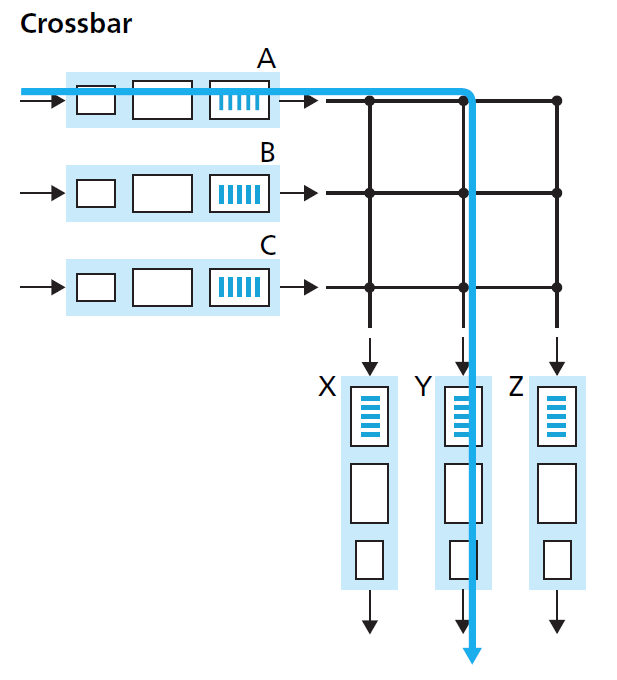
\includegraphics[scale=0.3]{Img-04-01-Crossbar}
\centering
\caption{Crossbar switch}
\label{fig:fig-04-01}
\end{figure}
A crossbar switch is an interconnection network consisting of 2\textit{N}buses that connect \textit{N} input ports to \textit{N} output ports, as shown in figure \ref{fig:fig-04-01}. Each vertical bus intersects each horizontal bus at a crosspoint, which can be opened or closed at any time by the switch fabric controller (whose logic is part of the switching fabric itself). When a packet arrives from port A and needs to be forwarded to port Y, the switch controller closes the crosspoint at the intersection of buses A and Y, and port A then sends the packet onto its bus, which is picked up (only) by bus Y. Note that a packet from port B can be forwarded to port X at the same time, since the A-to-Y and B-to-X packets uses different input and output buses.

\item
Let's new consider these queues in a bit more detail, since as these queues grow large, the router's memory can eventually be exhausted and \textbf{packet loss} will occur when no memory is available to store arriving packets.

\item
A consequence of output queuing is that a \textbf{packet scheduler} at the output port must choose one packet among those queued for transmission. This selection might be done on a simple basis, such as first-come-first-served (FCFS) scheduling, or a more sophisticated scheduling discipline such as weighted fair queuing (WFQ), which shares the outgoing link fairly among the different end-to-end connections that have packets queued for transmission.

\item
Similarly, if there is not enough memory to buffer an incoming packet, a decision must be made to either drop the arriving packet (a policy known as \textbf{drop-tail}) or remove one or more already-queued packets to make room for the newly arrived packet. In some cases, it may be advantageous to drop (or mark the header of) a packet \textit{before} the buffer is full in order to provide a congestion signal to the sender. A number of packet-dropping and -marking policies (which collectively have become known as \textbf{active queue management (AQM)} algorithms) have been proposed and analyzed. One of the most widely studied and implemented AQM algorithms is the \textbf{Random Early Detection (RED)} algorithm.

\item
A a queued packet in an input queue must wait for transfer through the fabric (even though its output port is free) because it is blocked by another packet at the head of the line, this phenomenon is known as \textbf{head-of-line (HOL) blocking} in an input-queued switch

\item
The network-wide routing control plane is thus decentralized---with different pieces (e.g., of a routing algorithm) executing at different routers and interacting by sending control messages to each other.

\item
Additionally, router and switch vendors bundle their hardware data plane and software control plane together into closed (but inter-operable) platforms in a vertically integrated product.

\item
Recently, a number of researchers have begun exploring new router control plane architectures in which part of the control plane is implemented in the routers (e.g., local measurement/reporting of link state, forwarding table installation and maintenance) along with the data plane, and part of the control plane can be implemented externally to the router (e.g., in a centralized server, which could perform route calculation). A well-defined API dictates how these two parts interact and communicate with each other.

\item
The Internet's network layer has three major components. The first component is the IP protocol. The second major component is the routing component, which determines the path a datagram follows from source to destination. The final component of the network layer is a facility to report errors in datagrams and respond to requests for certain network-layer information.

\item
The key fields in the IPv4 datagram are the following:
\begin{itemize}
\item\textit{Version number.}
\item\textit{Header length.}
\item\textit{Type of service.}
\item\textit{Datagram length.}
\item\textit{Identifier, flags, fragmentation offset.}
\item\textit{Time-to-live.}
\item\textit{Protocol.}
\item\textit{Header checksum.}
\item\textit{Source and destination IP addresses.}
\item\textit{Options.}
\item\textit{Data (payload).}
\end{itemize}

\item
The header checksum is computed by treating each 2 bytes in the header as a number and summing these numbers using 1s complement arithmetic. Note that the checksum must be recomputed and stored again at each router, as the TTL field, and possibly the options field as well, may change.\\
A question often asked at this point is, why does TCP/IP perform error checking at both the transport and network layers? There are several reasons for this repetition. First, note that only the IP header is checksummed at the IP layer, while the TCP/UDP checksum is computed over the entire TCP/UDP segment. Second, TCP/UDP and IP do not necessarily both have to belong to the same protocol stack.

\item
The maximum amount of data that a link-layer frame can carry is called the maximum transmission unit (MTU). Because each IP datagram is encapsulated within the link-layer frame for transport from one router to the next router, the MTU of the link-layer protocol places a hard limit on the length of an IP datagram.\\
The solution is to fragment the data in the IP datagram into two or more smaller IP datagrams, encapsulate each of these smaller IP datagrams in a separate link-layer frame; and send these frames over the outgoing link. Each of these smaller datagrams is referred to as a \textbf{fragment}.\\
To allow the destination host to perform these reassembly tasks, the designers of IP (version 4) put \textit{identification}, \textit{flag}, and \textit{fragmentation offset} fields in the IP datagram header.

\item
An IP address is technically associated with an interface, rather than with the host or router containing that interface.

\item
These addresses are typically written in so-called \textbf{dotted-decimal notation}, in which each byte of the address is written in its decimal form and is separated by a period (dot) from other bytes in the address.

















\end{itemize}